\subsection{FHR Benchmark Specifications}

\subsection{FHR Benchmark Results}

\begin{frame}
    \frametitle{FHR Benchmark Phase I-A Results}
    \begin{table}
        \caption{FHR Benchmark Phase I-A (2D assembly steady state model) results 
        \cite{chee_arfcfhr-benchmark_2021}.}
        \only<1>{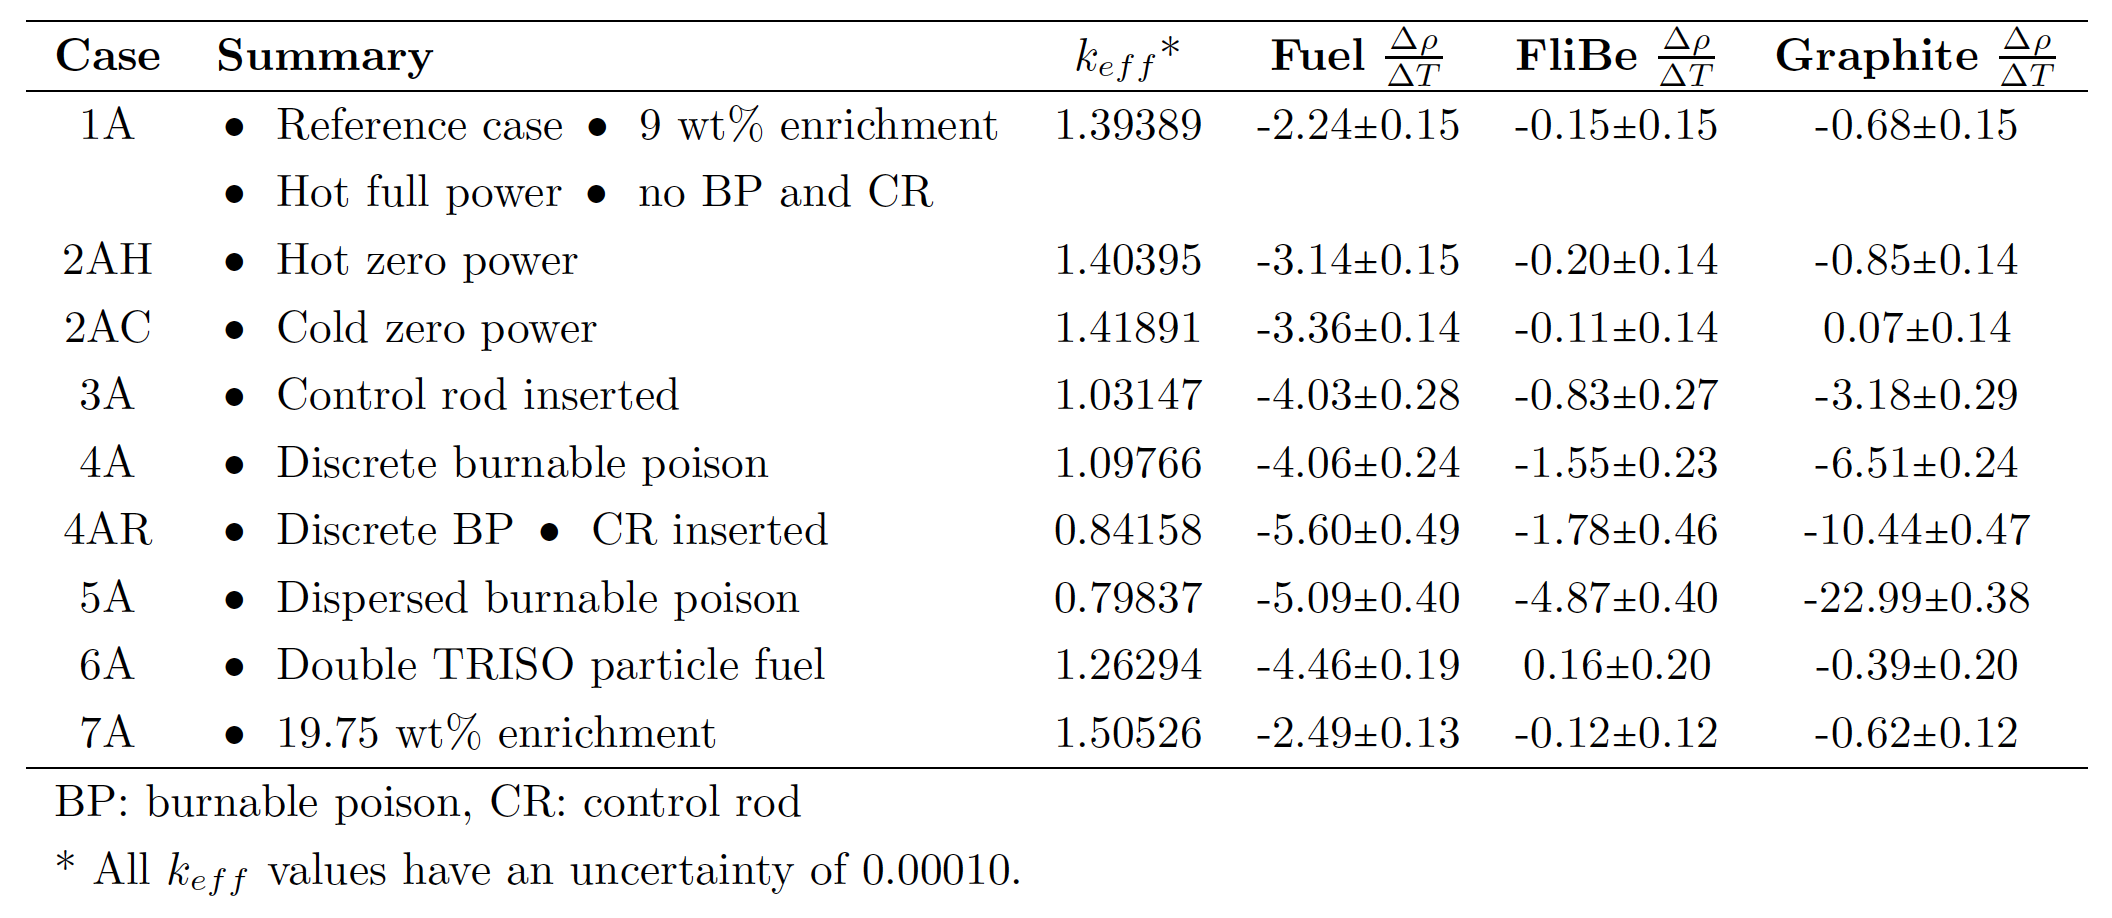
\includegraphics[width=\linewidth]{figures/benchmark-coeff-results.png}}
        \only<2>{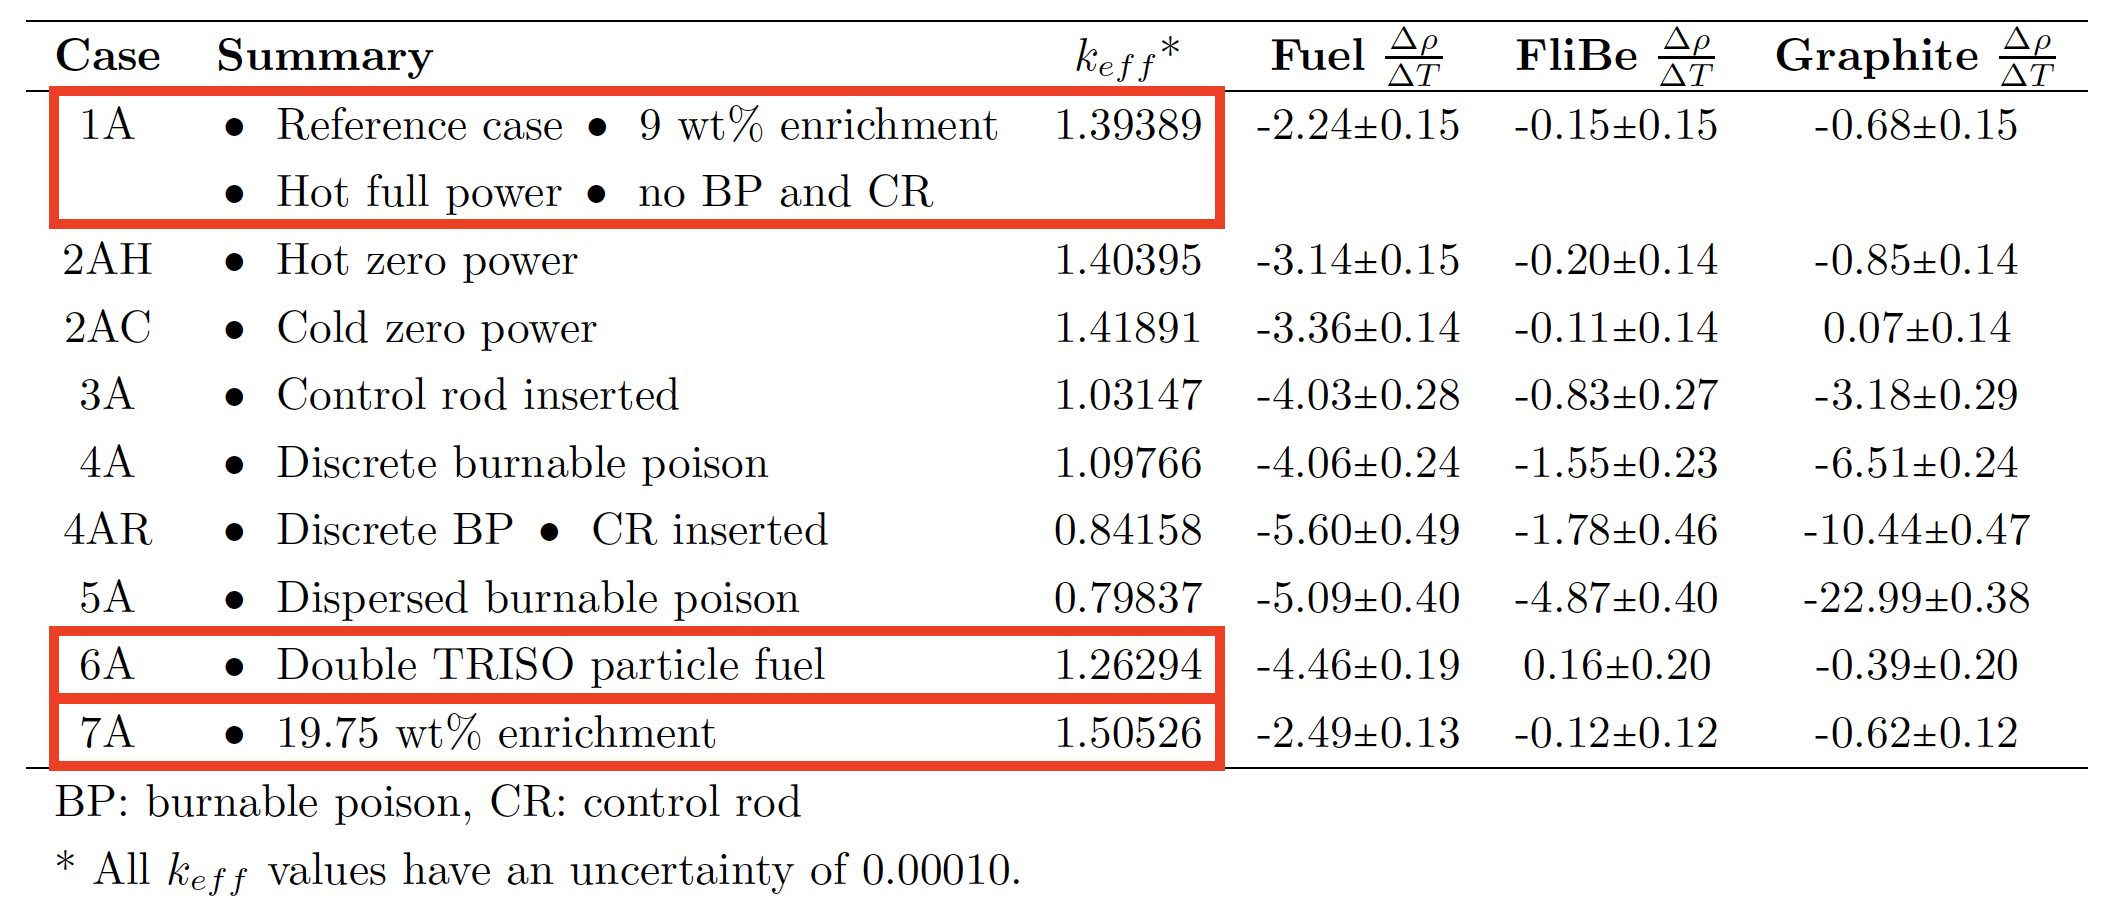
\includegraphics[width=\linewidth]{figures/benchmark-coeff-results-annotated.png}} 
        \only<3>{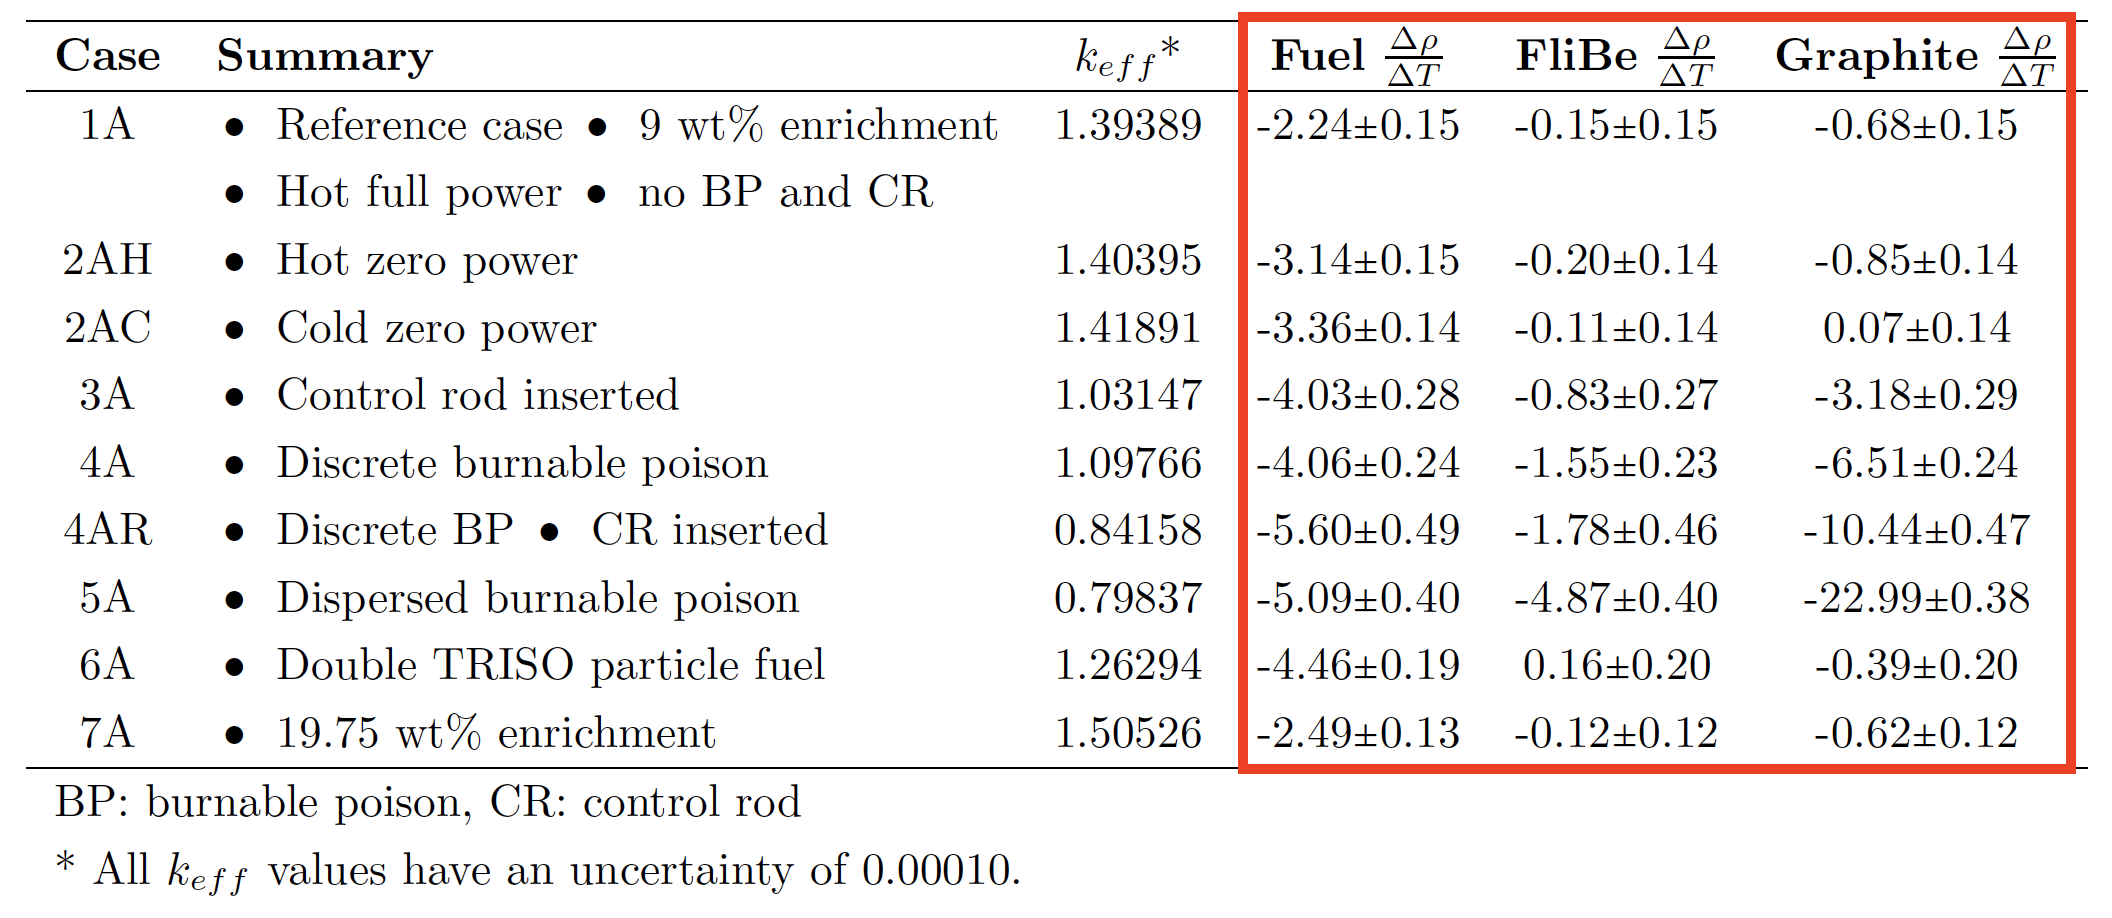
\includegraphics[width=\linewidth]{figures/benchmark-coeff-results-annotated2.png}} 
    \end{table}
    \vspace{-0.3cm}
    \only<1>{500 active cycles, 100 inactive cycles, and 200000 neutrons
    UIUC's BlueWaters supercomputer with 64 XE nodes}
    \only<2>{\textbf{Increased fuel packing does not always correspond with increased keff 
    due to spatial self-shielding effects.}}
\end{frame}

\begin{frame}
    \frametitle{FHR Benchmark Phase I-A Results}
    \begin{columns}
        \begin{column}{0.6\textwidth}
            \begin{figure}
                \centering
                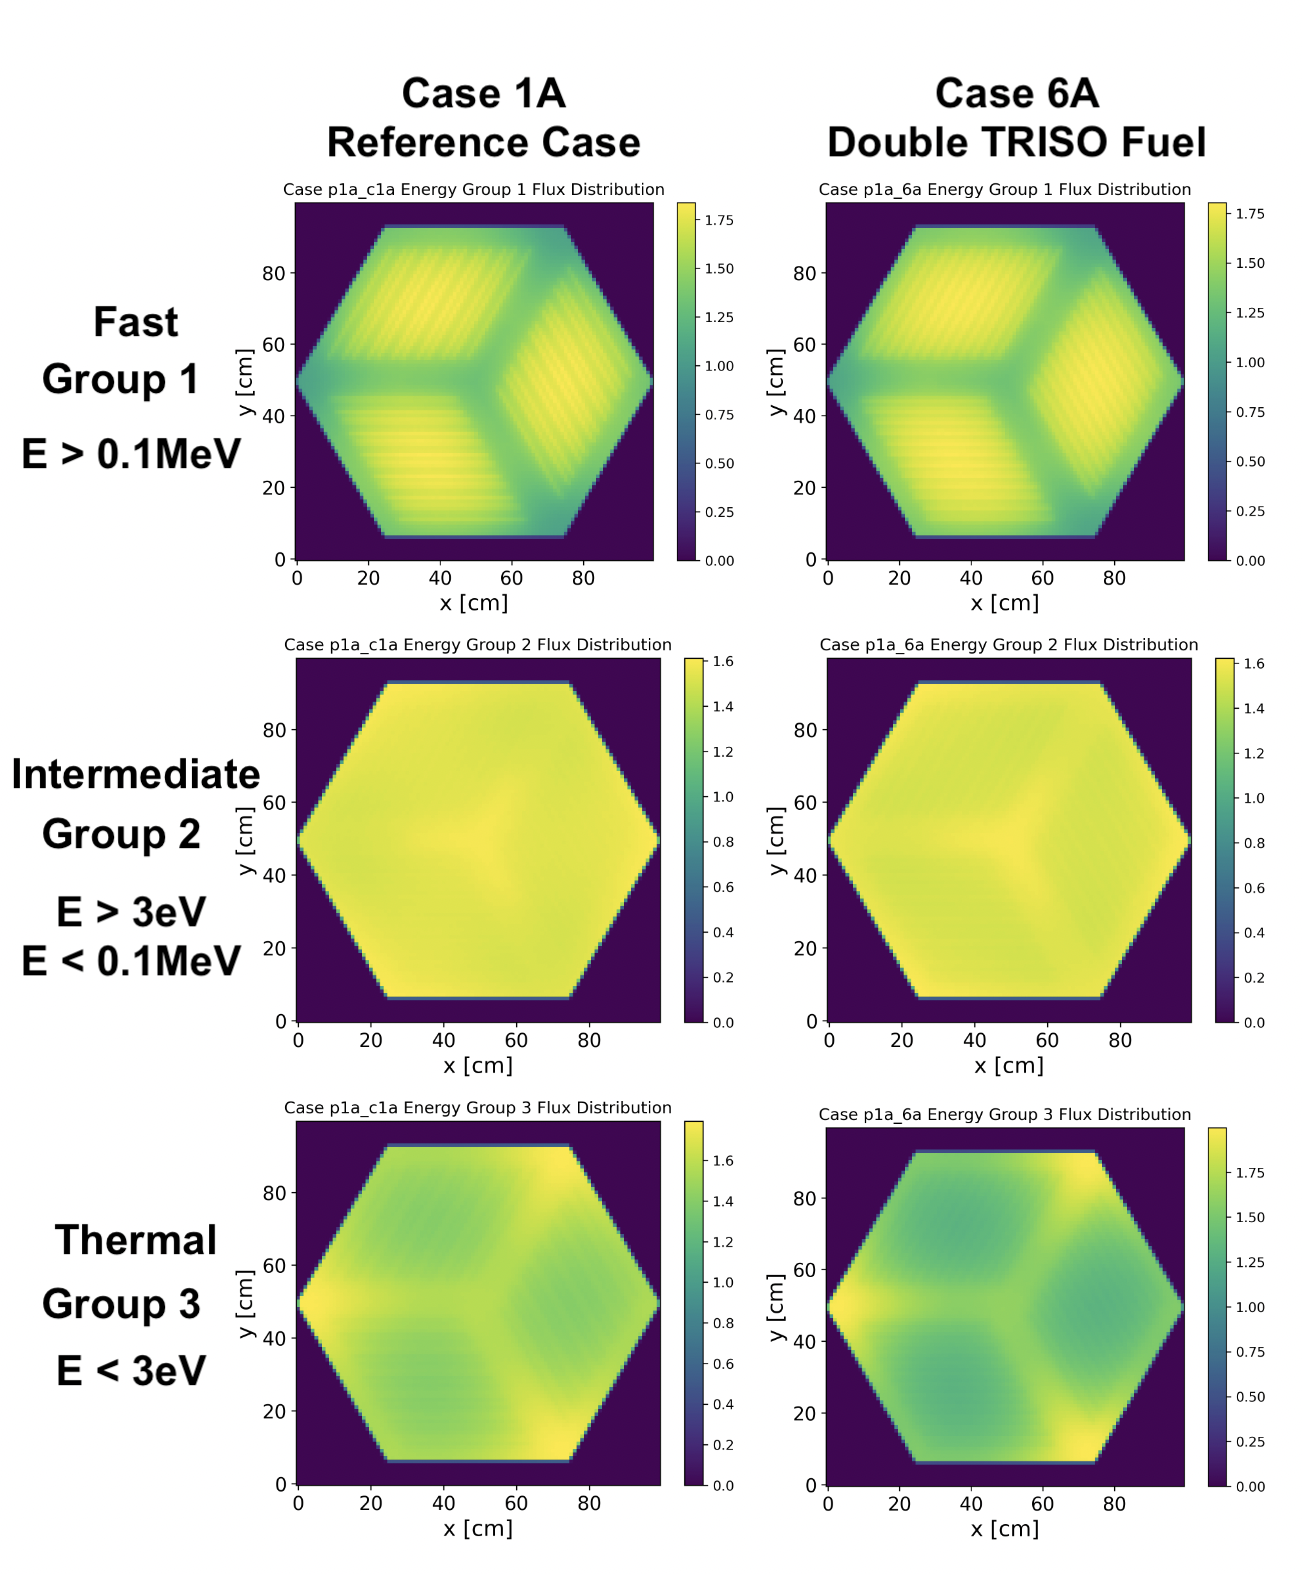
\includegraphics[width=0.8\linewidth]{figures/phase1a-flux-vert.png} 
                \caption{FHR Benchmark neutron flux distribution.}
            \end{figure}
        \end{column}
        \begin{column}{0.5\textwidth}
            Key Takeaways 
            \begin{itemize}
                \item Peak in Group 1 fast neutrons born in assembly center. Fast 
                neutrons are moderated in graphite matrix and structure 
                \item Self-shielding neutrons are more likely absorbed at the fuel 
                regions at the assembly's sides
                \item Outer sides absorb these neutrons and geometrically 
                shield the assembly's center from neutron flux, resulting in dip in 
                thermal Group 3 flux in the assembly's center
            \end{itemize}
        \end{column}
    \end{columns}
\end{frame}

\begin{frame}
    \frametitle{FHR Benchmark Phase I-A Results}
    In an ANS M$\&$C 2021 conference paper we compared FHR benchmark participants' 
    Phase I-A $k_{eff}$ results. 
    \begin{figure}[]
        \centering
        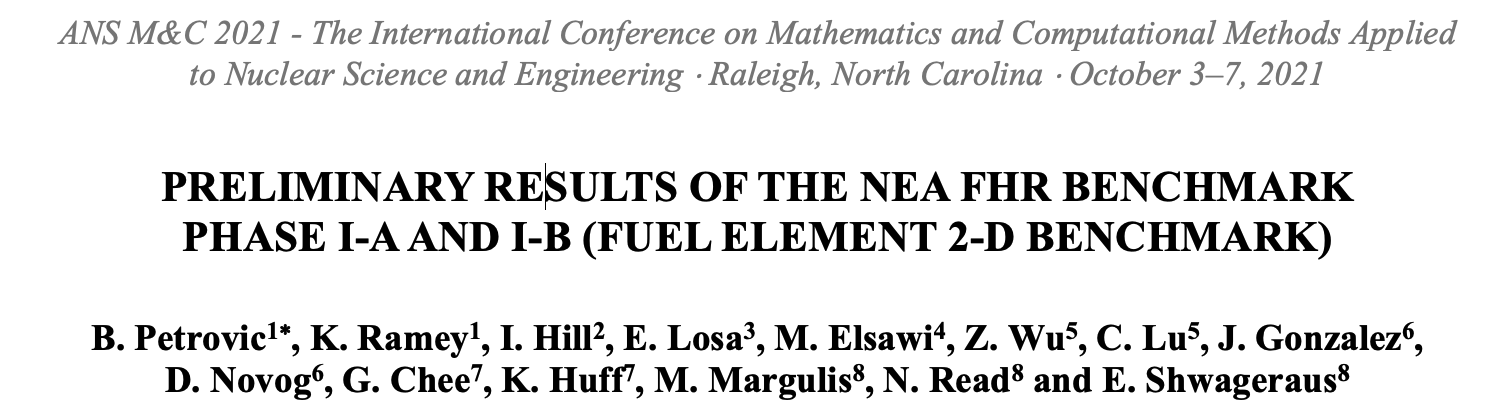
\includegraphics[width=0.85\linewidth]{figures/mnc.png} 
        \caption{FHR benchmark paper presented at M$\&$C 2021 
        \cite{petrovic_preliminary_2021}.}
    \end{figure}

    The standard deviation between participants for each case was in the 231 to 514 
    pcm range, \textbf{acceptable and notably close} given a blind benchmark.

    \vspace{0.2cm}
    This gives \textbf{confidence to the AHTR base model's accuracy}, as I 
    proceed to optimize the AHTR for non-conventional geometries. 
\end{frame}
